% airgap-rca: working manuscript. Compile with pdfLaTeX.
% Updated 2026-09-27: Product_A data, scenarios, and semantic retrieval.
% LLM, verification, and benchmark results remain pending.

\documentclass[conference]{IEEEtran}

\usepackage[T1]{fontenc}
\usepackage{amsmath,amssymb}
\usepackage{graphicx,booktabs,array,tabularx}
\usepackage{xcolor,tikz}
\usetikzlibrary{arrows.meta,positioning,shapes.geometric}
\usepackage{listings}
\usepackage{xurl}
\usepackage[hidelinks]{hyperref}

\definecolor{accent}{HTML}{245A73}
\definecolor{pale}{HTML}{EDF3F6}

\newcommand{\system}{\textsc{airgap-rca}}
\newcommand{\pending}{\textcolor{accent}{\textit{Pending}}}

\newcommand{\draftnote}[1]{%
\par\smallskip\noindent
\colorbox{pale}{%
\parbox{\dimexpr\columnwidth-2\fboxsep\relax}{%
\small\textbf{Draft task.} #1}}%
\par\smallskip}

\newcommand{\placeholder}[2]{%
\noindent\fbox{%
\parbox[c][#1][c]{0.94\columnwidth}{%
\centering\small\textcolor{accent}{#2}}}}

\newcolumntype{Y}{>{\raggedright\arraybackslash}X}

\lstset{
    basicstyle=\ttfamily\scriptsize,
    breaklines=true,
    columns=fullflexible,
    frame=single,
    rulecolor=\color{accent},
    showstringspaces=false
}

\pagestyle{plain}

\begin{document}

\title{Sovereign Root Cause Analysis:
Grounded Log Triage on Air-Gapped Edge Accelerators,
with a Cross-Silicon Characterisation}

\author{
\IEEEauthorblockN{Kayman Srinivasan}
\IEEEauthorblockA{
Working manuscript --- September 2026\\
Affiliations and co-authors to be confirmed\\[0.5em]
Supervisor: Kother Badushah\\
Solutions Architect (Semicon and AI), UST
}
}

\maketitle

\begin{abstract}
\textbf{Working abstract; evaluation pending.}
Engineering teams operating under strict data residency constraints
need methods for investigating failures without exporting their logs.
This project develops a local evidence-grounded triage pipeline for
semiconductor automated test equipment (ATE). The current prototype
uses generated Product\_A wafer-sort logs covering five lots,
35 wafers, and 3,920 devices under test (DUTs), with a simplified
flow comprising Continuity, IDD\_Static, and Scan. Six historical
case scenarios extend selected observations with synthetic
investigation, action, and retest records informed by ATE engineer
guidance. A seventh observation-only case represents an incoming
failure. The implemented retrieval stage stores 384-dimensional
MiniLM observation embeddings in Chroma, ranks eligible historical
observations, and assembles their linked case histories.
Local language-model generation, deterministic answer verification,
and refusal remain planned components. Evaluation on Jetson AGX Orin
and Qualcomm RB3 Gen 2 will examine answer quality, latency,
throughput, power, and energy under documented configurations.
Current development establishes data preparation and evidence
assembly; it does not establish diagnostic accuracy, confirmed
physical causes, or cross-platform performance.
\end{abstract}

\begin{IEEEkeywords}
root cause analysis, log triage, air-gapped inference,
retrieval-augmented generation, selective prediction, edge computing
\end{IEEEkeywords}

\section{Introduction}

Machine logs record events that can help engineers reconstruct the
sequence leading to a failure. A useful triage assistant must locate
relevant events, relate them to a specific question, and provide
evidence that a human can inspect. In environments that prohibit
external processing of engineering data, retrieval and generation
must operate locally. This project treats disconnected execution
as an experimental requirement.

The intended output is a short ranked list of supported candidate
causes, not an unrestricted explanation. A recorded symptom does
not necessarily establish a physical root cause. For example,
a Continuity failure alone cannot distinguish a DUT-related
abnormality from an interface or contact problem. The system must
preserve this uncertainty and refuse questions that require
absent evidence.

\subsection{Research questions}

\begin{itemize}
\item \textbf{RQ1: Reliability.}
How often does the system accept an incorrect answer,
and what coverage does it retain?

\item \textbf{RQ2: Component contribution.}
How do historical-case selection, verification, and refusal
affect quality and latency?

\item \textbf{RQ3: Platform trade-offs.}
Under documented, comparable settings, how do the two execution
platforms differ in latency, throughput, and energy?
\end{itemize}

\subsection{Planned contributions and scope}

The planned contributions are a reproducible offline pipeline,
a reviewed question-and-evidence evaluation set, and a cross-platform
characterisation. The initial prototype is restricted to three
wafer-sort tests: Continuity (Open/Short), IDD\_Static, and Scan.
This reduced scope follows project guidance to limit log complexity
while developing the evidence-to-answer workflow.

The active data comprise generated Product\_A observations and
engineer-informed synthetic case histories. Fine-tuning, a chat
interface, and autonomous recovery are outside the core study.
The current scenarios demonstrate pipeline behaviour; they do not
establish manufacturing failure rates, physical root causes,
or performance on other products, test programs, or BIST failures.

\draftnote{
Substantiate the motivation with primary literature.
Do not claim a percentage of debugging time or global novelty
without supporting sources.
}

\section{Related Work}

\subsection{Log analysis and failure diagnosis}

Loghub provides public system-log collections and their
provenance~\cite{loghub}. Candidate selection must distinguish
anomaly labels from cause labels. In particular, the Hadoop
dataset documents injected failure scenarios~\cite{hadoop},
but reported label inconsistencies require incident-level
review~\cite{hadooplabels}. Hadoop was explored during initial
data selection but is not the active prototype dataset;
the current implementation uses the generated Product\_A
data described below.

\subsection{Evidence-grounded generation}

\draftnote{
Weeks 2--3: add verified primary papers on retrieval-augmented
generation, attribution, and abstention. Compare their evidence
guarantees with this system. Separate citation existence,
textual relevance, and causal correctness.
}

\subsection{Offline inference and platform evaluation}

\draftnote{
Weeks 2--4: review primary work on local inference and energy
measurement. Describe the gap supported by that review;
do not equate an IEEE layout with publication readiness.
}

\section{System Design}

\subsection{Execution boundary and provenance}

Figure~\ref{fig:architecture} distinguishes implemented preparation
and retrieval from the planned answer-generation stages.
A connected development machine prepares the assets.
Full disconnected execution on the target boards remains
to be demonstrated.

The original generated wafer logs are treated as immutable evidence.
The chunker produces one observation per DUT, preserving the complete
source block, relative source path, SHA-256 checksum, and inclusive
one-based line range. Derived chunks retain identifiers and observed
test outcomes without assigning a cause. Investigation, action,
and retest records are stored separately as synthetic JSON evidence
linked to the corresponding observation.

Raw-log citations can use filenames and original line ranges.
Scenario records instead carry stable record identifiers,
case identifiers, source JSON paths, and review-status information.
The evidence bundle preserves these references for later generation
and verification.

\begin{figure}[t]
\centering
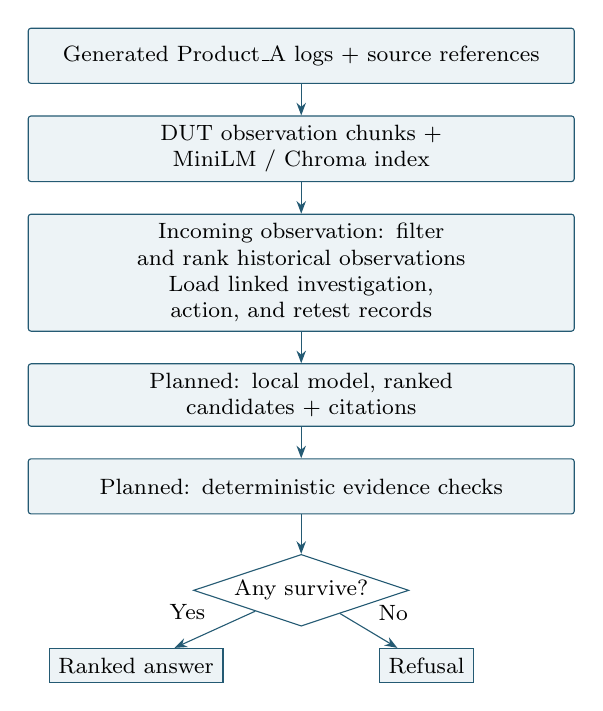
\begin{tikzpicture}[
    node distance=4mm,
    font=\footnotesize,
    box/.style={
        draw=accent,
        rounded corners=1pt,
        align=center,
        text width=6.7cm,
        minimum height=7mm,
        fill=pale
    },
    arr/.style={
        -{Stealth[length=1.6mm]},
        draw=accent
    }
]

\node[box] (raw)
{Generated Product\_A logs + source references};

\node[box,below=of raw] (idx)
{DUT observation chunks + MiniLM / Chroma index};

\node[box,below=of idx] (ret)
{Incoming observation: filter and rank historical observations\\
Load linked investigation, action, and retest records};

\node[box,below=of ret] (gen)
{Planned: local model, ranked candidates + citations};

\node[box,below=of gen] (ver)
{Planned: deterministic evidence checks};

\node[
    draw=accent,
    diamond,
    aspect=3,
    align=center,
    below=5mm of ver,
    inner sep=1pt
] (gate)
{Any survive?};

\node[
    draw=accent,
    fill=pale,
    align=center,
    below left=5mm and 3mm of gate
] (yes)
{Ranked answer};

\node[
    draw=accent,
    fill=pale,
    align=center,
    below right=5mm and 3mm of gate
] (no)
{Refusal};

\draw[arr] (raw)--(idx);
\draw[arr] (idx)--(ret);
\draw[arr] (ret)--(gen);
\draw[arr] (gen)--(ver);
\draw[arr] (ver)--(gate);

\draw[arr] (gate)--node[above left]{Yes}(yes);
\draw[arr] (gate)--node[above right]{No}(no);

\end{tikzpicture}

\caption{
Current prototype and intended continuation.
Data preparation, observation indexing, and linked evidence
assembly are implemented. LLM generation, answer verification,
and refusal are pending.
}
\label{fig:architecture}
\end{figure}

\subsection{Local semantic retrieval and case-history assembly}

The current embedding model is \texttt{all-MiniLM-L6-v2},
which maps text to 384-dimensional vectors~\cite{minilmcard}.
The Python scripts invoke Chroma's
\texttt{DefaultEmbeddingFunction} locally and explicitly supply
the resulting vectors to the collection. The project dependency
is pinned to Chroma 1.5.9. No model fine-tuning is performed
for this prototype.

The persistent Chroma collection,
\texttt{product\_a\_observations}, stores all 3,920 DUT observation
texts, their embeddings, and metadata identifying the DUT and
its source chunk~\cite{chroma}. The same encoder is used for
an incoming observation. The current path uses vector retrieval
with metadata filtering; it does not combine vector and
keyword scores.

The case-history demonstration first constructs a mapping from
DUT identifiers to the six complete historical scenarios.
It selects cases with the same failed test as the incoming
observation, then filters the Chroma query to those DUT identifiers.
It requests up to three matches, or fewer when fewer eligible
cases exist. For Case~07, the filter leaves two historical
Continuity cases. Therefore, this demonstration ranks two eligible
observations rather than searching all 3,920 records
without restriction.

For each match, the script loads the associated observation,
investigation, action, and retest JSON records. The 18 historical
follow-up records are not separately embedded in this
implementation. Case and observation identifiers are checked
before the evidence is assembled. The output bundle retains
the incoming observation separately from the historical records
and includes citation identifiers, source paths, and
synthetic-data status.

An initial development run assembled Case~07 with the histories
of Cases~01 and~02. This confirms operation of the
retrieval-and-linking path for that example, not general retrieval
accuracy. Returned vector distances indicate relative proximity
within the configured index; they are not probabilities of a cause.
Historical outcomes must not be attributed to the incoming DUT
without current-incident evidence.

\subsection{Structured generation}

The planned generator will receive the question or incoming
observation and the assembled evidence bundle. It is intended
to return at most three ranked candidates using a fixed schema.
Each candidate separates the proposed cause from exact quoted
evidence and references. Self-reported confidence is not treated
as a calibrated probability.

\begin{lstlisting}[
    float=t,
    caption={Proposed output fields; schema illustration only.},
    label={lst:schema}
]
{
  "status": "answer | refusal",
  "candidates": [{
    "rank": "integer",
    "cause": "narrow supported claim",
    "confidence": "optional uncalibrated score",
    "citations": [{
      "source_id": "allowed source identifier",
      "line_start": "original line number",
      "line_end": "original line number",
      "quote": "exact source text"
    }]
  }],
  "refusal_reason": "when applicable"
}
\end{lstlisting}

Listing~\ref{lst:schema} describes proposed field types using strings;
it is not an executable response or a formal JSON Schema.
Before integration, the citation schema must also represent
scenario record identifiers and JSON source locations alongside
raw-log line references. Parse failures must be logged.
Logs are untrusted data, never instructions to the model or host.
The final LLM checkpoint, runtime, and decoding configuration
remain to be verified.

\subsection{Deterministic verification and refusal}

This stage is not yet implemented. For candidate $j$, define
indicators for schema validity $s_j$, allowed-source membership
$a_j$, valid line bounds $b_j$, quote fidelity $q_j$, and the
fixed relevance policy $r_j$. A proposed gate is

\begin{equation}
V_j=s_j a_j b_j q_j r_j,\qquad
\mathrm{refuse}\ \text{if}\ \sum_j V_j=0.
\end{equation}

All citations and atomic claims in a retained candidate must
satisfy the selected policy. Record each rejection reason and
preserve surviving order. Exact-quote and line-bound checks
establish integrity; term overlap does not prove entailment
or causation. Cause correctness therefore requires independent
evaluation. Execution failures must not be silently reclassified
as successful refusals.

\draftnote{
Week 3: specify the actual relevance rule, negation handling,
multiple-citation policy, invalid-output policy, and any retry
budget. Define source-specific checks for JSON scenario records
as well as raw-log lines. Include examples the verifier
mistakenly accepts.
}

\section{Platforms and Experimental Setup}

\subsection{Hardware and execution configuration}

Populate Table~\ref{tab:hardware} from dated board inspection
records. Confirm accelerator execution with runtime evidence
and report CPU fallback. A successful process on a board does
not establish NPU use. Match the base checkpoint, tokenizer,
context budget, and decoding configuration. Report weight and
activation precision and quantisation method; equal bit width
alone is not equivalence.

\begin{table}[t]
\caption{Platform configuration record. No specifications verified yet.}
\label{tab:hardware}
\centering\footnotesize
\begin{tabularx}{\columnwidth}{@{}Yll@{}}
\toprule
Configuration & Jetson AGX Orin & RB3 Gen 2\\
\midrule
Module, RAM, storage & \pending & \pending\\
OS, kernel, SDK & \pending & \pending\\
Runtime, backend & \pending & \pending\\
Checkpoint, tokenizer & \pending & \pending\\
Weights / activations & \pending & \pending\\
Quantisation method & \pending & \pending\\
Context / output budget & \pending & \pending\\
Power mode / clocks & \pending & \pending\\
Cooling / temperature & \pending & \pending\\
Power measurement & \pending & \pending\\
\bottomrule
\end{tabularx}
\end{table}

\subsection{Dataset and answer-key construction}

\subsubsection{Generated Product\_A observations}

The active dataset contains five lots, seven wafers per lot,
and 112 DUTs per wafer:

\[
5 \times 7 \times 112 = 3{,}920 \text{ DUTs}.
\]

The 35 readable wafer files are accompanied by structured DUT
metadata, a generation configuration, a coordinate template,
a manifest of file checksums, and a validation report.
Matching STDF exports provide an alternative representation
of the same observations; they do not represent additional
tested devices.

The earlier A595 example supplied the readable format,
selected test definitions, a coordinate layout, and example
current limits. Product\_A measurements and outcomes were
generated from the included configuration; no physical
Product\_A device was tested. The outcome quotas are chosen
demonstration values rather than observed manufacturing yield.

Each DUT begins with test~100, \texttt{Open/Short-}.
A pass permits test~210, \texttt{IDD\_Static};
another pass permits test~606, \texttt{SCAN Test}.
Testing stops at the first failure.
Table~\ref{tab:producta} summarises the generated outcomes
and the corresponding executed paths.

\begin{table}[t]
\caption{
Generated Product\_A observations.
Counts are dataset construction values,
not measured production yield.
}
\label{tab:producta}
\centering\footnotesize
\begin{tabularx}{\columnwidth}{@{}Yrrl@{}}
\toprule
Outcome & Bin & DUTs & Tests executed\\
\midrule
All tests pass & 1 & 3,528 & 100, 210, 606\\
Continuity failure & 4 & 98 & 100\\
IDD\_Static failure & 3 & 98 & 100, 210\\
Scan failure & 2 & 196 & 100, 210, 606\\
\midrule
Total & -- & 3,920 & --\\
\bottomrule
\end{tabularx}
\end{table}

The stopping rule yields 3,920 Continuity, 3,822 IDD\_Static,
and 3,724 Scan results: 11,466 executed test results in total.
The prototype IDD\_Static pass condition is strictly between
35 and 55~mA. These limits and the pin and scan-pattern settings
are synthetic configuration assumptions, not validated
Product\_A specifications.

An independent validator reads back the generated logs and
checks their consistency with the configuration, metadata,
and manifest. These checks establish internal dataset
consistency; they do not validate the physical realism of
every generated failure.

\subsubsection{Engineer-informed historical scenarios}

Six selected DUT observations are extended into historical
scenarios: two Continuity cases, two IDD\_Static cases,
and two Scan cases. Each case has four linked records:

\begin{enumerate}
\item \textbf{Observation:}
the existing generated DUT result and source references.

\item \textbf{Investigation:}
possible explanations, selected checks, and simulated findings.

\item \textbf{Action:}
the simulated response to those findings.

\item \textbf{Retest:}
simulated subsequent results, a supported scenario conclusion,
and remaining limitations.
\end{enumerate}

ATE engineer Ansari provided guidance on possible causes,
checks to distinguish DUT-related problems from interface
or tester problems, and useful action/retest evidence.
The subsequently authored findings and outcomes are simulated
rather than physically observed. Engineer guidance and synthetic
outcome review status remain distinct: the new outcomes have
not been certified as engineer-reviewed diagnoses.

The six cases include both recovery after interface or setup
changes and persistent DUT-associated failures whose exact
physical mechanisms remain unresolved. This prevents every
history from implying that a successful repair or a precise
physical diagnosis is available.

\subsubsection{Incoming case and evidence separation}

Case~07 is an additional synthetic incoming observation,
identified as \texttt{Product\_A-L06-W01-D001}.
It reports a Continuity failure on TSTIN and contains no
investigation, action, or retest. It is not one of the
3,920 indexed DUTs from Lots~L01--L05 and does not represent
a sixth generated production lot.

The scenario set therefore contains 24 historical records
and one incoming observation, for 25 JSON files in total.
Case~07 is marked query-only and excluded from historical
retrieval. Its source is the authored observation JSON rather
than a fabricated wafer-log reference. Completed historical
case outcomes may support possible causes and suggested checks,
but they do not establish what happened to this incoming DUT.

\subsubsection{Planned evaluation set}

These seven scenarios are development examples, not a completed
diagnostic benchmark. The proposed evaluation target remains
at least 50 answerable questions and at least 10 refusal cases,
subject to sufficient reviewed evidence. Each item will need
an answerability label, accepted claims, source references,
and a review rationale.

Historical reference evidence must be separated from
evaluation-incident outcomes and answer keys. Split by incident
rather than merely rewording the same question, and report
dependence among questions derived from a common scenario.
Refusal cases should cover insufficient evidence and unsupported
claims of confirmation; missing confirmation need not prevent
a properly qualified cause suggestion. Synthetic evaluation
will measure behaviour within the authored scenarios,
not real-world physical diagnostic accuracy.

\draftnote{
Before evaluation, freeze the question set, scoring policy,
evidence available at each stage, review process, and exclusions.
No answer-accuracy or refusal results are available yet.
}

\subsection{Quality metrics and denominators}

Let $N$ denote all frozen questions, $N_A$ answerable questions,
and $N_U$ unanswerable questions. For question $i$, let $a_i$
indicate an accepted answer, $r_i$ a refusal, and $e_i$ an
execution error, with $a_i+r_i+e_i=1$. Let $z_i$ indicate
answerability and $c_i^{(k)}$ indicate that a reviewed correct
cause appears in the first $k$ returned candidates.
Refusals and errors have $c_i^{(k)}=0$.

\begin{align}
\mathrm{Acc@}k &=
\frac{\sum_i z_i c_i^{(k)}}{N_A},
\quad k\in\{1,3\},\\
\mathrm{FAR} &=
\frac{\sum_i a_i(1-c_i^{(1)})}{N},\\
\mathrm{AnsweredError} &=
\frac{\sum_i a_i(1-c_i^{(1)})}{\sum_i a_i},\\
\mathrm{Coverage} &=
\frac{\sum_i a_i}{N},\qquad
\mathrm{RefusalRate}=\frac{\sum_i r_i}{N},\\
\mathrm{CorrectRefusal} &=
\frac{\sum_i(1-z_i)r_i}{N_U}.
\end{align}

An accepted answer on an unanswerable case is wrong under
the reviewed policy. A zero denominator is reported as not
applicable, never zero. Also report execution-error rate and
the fraction of answered questions containing any incorrect
candidate, even when the first cause is correct. The exact
scoring policy remains to be agreed before evaluation.

For generated citations $C_g$ and citations passing
the verifier $C_v$,

\begin{equation}
\mathrm{CitationPassRate}=\frac{|C_v|}{|C_g|}.
\end{equation}

Report this before filtering and report post-filter integrity
separately. Call it a verifier pass rate unless independent
review supports a stronger validity claim. Pair FAR with
coverage to expose a system that obtains few errors by
refusing almost everything. Include uncertainty intervals;
zero observed errors is not proof of zero deployment risk.

\subsection{Timing, throughput, power, and energy}

For each request, end-to-end latency covers question submission
through final verified output, including retrieval and any
retries. Report index-building and cold-start costs separately.
Fix warm-up, repetition, request ordering, concurrency,
output-token counting, and thermal-state procedures
before final runs.

\begin{align}
L_i &= t_{\mathrm{final},i}-t_{\mathrm{submit},i},\\
\mathrm{TPS}_{\mathrm{decode}} &=
\frac{n_{\mathrm{out}}-1}
{t_{\mathrm{last}}-t_{\mathrm{first}}}.
\end{align}

The decode formula requires at least two output tokens.
Record time to first token separately and state whether
token timing is provided by the runtime or observed externally.
Do not estimate throughput from nominal model specifications.

Measure power over the same system boundary on both boards.
For sampled power, integrate using timestamps:

\begin{equation}
E_i\approx
\sum_{m=1}^{M_i-1}
\frac{P_{i,m}+P_{i,m+1}}{2}
\left(t_{i,m+1}-t_{i,m}\right).
\end{equation}

Power is in watts and time in seconds, giving joules. Then

\begin{align}
\bar E &=
\frac{1}{N_{\mathrm{measured}}}\sum_i E_i,\\
\bar P_{\mathrm{active}} &=
\frac{\sum_i E_i}{\sum_i L_i},\\
\mathrm{Cost}_{1000} &=
\frac{1000\bar E}{3.6\times10^6}\,p_{\mathrm{kWh}}.
\end{align}

Use only matching measured intervals for average power.
The cost is electricity-only; state currency and tariff.
Report whether energy includes idle draw, startup, and refusals.
Report missing measurements rather than inventing estimates.

\subsection{Offline execution protocol}

Bundle weights, tokenizer assets, embeddings, wheels,
native libraries, runtime components, and documentation
with checksums. Disconnect all network paths, reboot,
and execute the recorded request sequence without manual repair.
Preserve startup logs and the exact bundle identity.
Record the initial week-1 smoke test separately from final
reproducibility tests.

\section{Results and Analysis}

\textbf{Diagnostic and cross-board evaluation remain pending.}
Completed data preparation and initial evidence assembly are
implementation milestones, not answer-quality or
hardware-performance measurements. Every pending cell and empty
chart is a holder, not a zero-valued result.
Tables~\ref{tab:quality}--\ref{tab:ablation} and
Figs.~\ref{fig:tradeoff}--\ref{fig:far} are reserved for
script-generated output.

\subsection{Quality and refusal behaviour}

% PLACEHOLDER ONLY: no experimental measurements.
\begin{table}[t]
\caption{Quality holders. Rates require explicit denominators and uncertainty.}\label{tab:quality}
\centering\footnotesize
\begin{tabularx}{\columnwidth}{@{}Yll@{}}\toprule
Metric & Jetson & RB3\\\midrule
Answerable / unanswerable count & \pending & \pending\\
Top-1 / top-3 accuracy (\%) & \pending & \pending\\
False answer rate (\%) & \pending & \pending\\
Error among answers (\%) & \pending & \pending\\
Any-wrong-candidate rate (\%) & \pending & \pending\\
Coverage / refusal rate (\%) & \pending & \pending\\
Correct refusal rate (\%) & \pending & \pending\\
Citation pass rate, pre-filter (\%) & \pending & \pending\\
Post-filter citation integrity (\%) & \pending & \pending\\
Execution-error rate (\%) & \pending & \pending\\
\bottomrule\end{tabularx}
\end{table}


\draftnote{
Weeks 3--5: interpret FAR alongside coverage and refusal success.
Discuss wrong secondary candidates and verifier false accepts.
Include uncertainty and counts, not only rounded percentages.
}

\subsection{Cross-platform performance}

% PLACEHOLDER ONLY: no experimental measurements.
\begin{table}[t]
\caption{Performance holders. Record repetitions and power boundary.}\label{tab:performance}
\centering\footnotesize
\begin{tabularx}{\columnwidth}{@{}Yll@{}}\toprule
Metric & Jetson & RB3\\\midrule
Latency: median / p95 (s) & \pending & \pending\\
Time to first token (s) & \pending & \pending\\
Decode throughput (tokens/s) & \pending & \pending\\
Average / peak power (W) & \pending & \pending\\
Mean energy per triage (J) & \pending & \pending\\
Electricity price (currency/kWh) & \pending & \pending\\
Cost per 1,000 (currency) & \pending & \pending\\
Cold-start / indexing time (s) & \pending & \pending\\
\bottomrule\end{tabularx}
\end{table}


\begin{figure}[t]
\centering
% PLACEHOLDER ONLY: no experimental measurements.
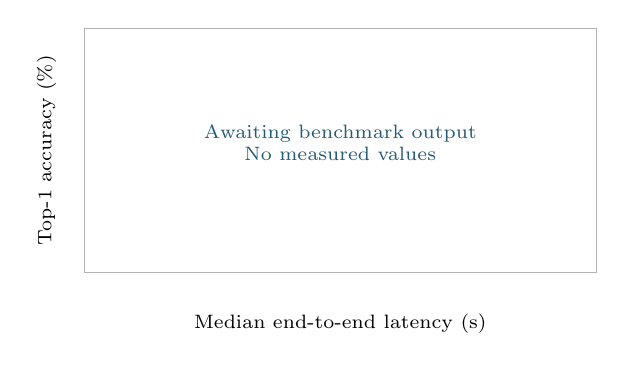
\begin{tikzpicture}[font=\scriptsize]
\draw[gray!60] (0,0) rectangle (6.5,3.1);
\node[align=center,text=accent] at (3.25,1.65) {Awaiting benchmark output\\No measured values};
\node[rotate=90] at (-0.48,1.55) {Top-1 accuracy (\%)};
\node at (3.25,-0.65) {Median end-to-end latency (s)};
\end{tikzpicture}

\caption{
Reserved accuracy--latency plot: one measured point per
platform/configuration. Use median end-to-end latency and
answerable-set top-1 accuracy; show uncertainty where supported.
No observations plotted.
}
\label{fig:tradeoff}
\end{figure}

\begin{figure}[t]
\centering
% PLACEHOLDER ONLY: no experimental measurements.
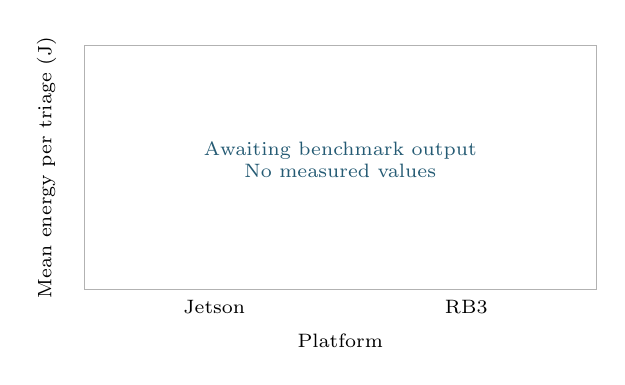
\begin{tikzpicture}[font=\scriptsize]
\draw[gray!60] (0,0) rectangle (6.5,3.1);
\node[align=center,text=accent] at (3.25,1.65) {Awaiting benchmark output\\No measured values};
\node[rotate=90] at (-0.48,1.55) {Mean energy per triage (J)};
\node at (3.25,-0.65) {Platform};
\node at (1.65,-0.22) {Jetson};
\node at (4.85,-0.22) {RB3};
\end{tikzpicture}

\caption{
Reserved energy comparison: mean measured joules per triage
on the same workload and power boundary, with uncertainty.
No observations plotted.
}
\label{fig:energy}
\end{figure}

\draftnote{
Weeks 4--5: explain runtime and quantisation deviations before
attributing differences to accelerator hardware.
Include p95 latency and measured peak power.
}

\subsection{Component ablations}

% PLACEHOLDER ONLY: no experimental measurements.
\begin{table}[t]
\caption{Ablation holders. J/R denotes separate Jetson and RB3 results in each cell. All entries await measurements.}
\label{tab:ablation}\centering\scriptsize
\begin{tabularx}{\columnwidth}{@{}Yccc@{}}\toprule
Configuration & FAR (\%) & Coverage (\%) & Acc@1 (\%)\\\midrule
Full pipeline & --/-- & --/-- & --/--\\
Without keywords & --/-- & --/-- & --/--\\
Without verification & --/-- & --/-- & --/--\\
Without refusal & --/-- & --/-- & --/--\\\bottomrule
\end{tabularx}
\end{table}


\begin{figure}[t]
\centering
% PLACEHOLDER ONLY: no experimental measurements.
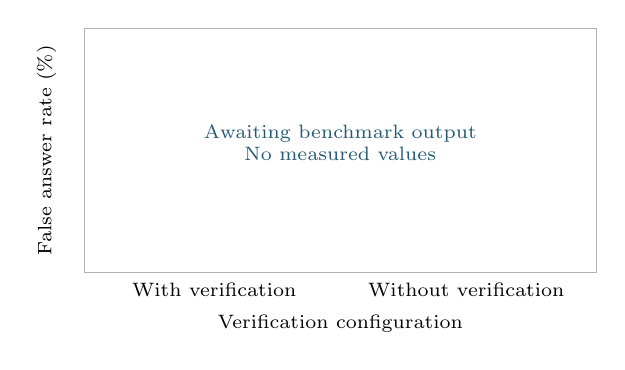
\begin{tikzpicture}[font=\scriptsize]
\draw[gray!60] (0,0) rectangle (6.5,3.1);
\node[align=center,text=accent] at (3.25,1.65) {Awaiting benchmark output\\No measured values};
\node[rotate=90] at (-0.48,1.55) {False answer rate (\%)};
\node at (3.25,-0.65) {Verification configuration};
\node at (1.65,-0.22) {With verification};
\node at (4.85,-0.22) {Without verification};
\end{tikzpicture}

\caption{
Reserved verification ablation: false answer rate with and
without verification, for each platform. Report coverage
alongside the plotted rate. No observations plotted.
}
\label{fig:far}
\end{figure}

Planned ablations will use the same frozen incidents and model
configuration. The current retrieval implementation already uses
vector search without keyword fusion. Verification and refusal
ablations can be defined once those stages are implemented.
A run without verification would bypass candidate filtering
while retaining schema handling; a run without refusal would
use an explicitly defined forced-answer policy.
Record exactly which stages change and distinguish replayed
candidate-output checks from end-to-end runs.

\draftnote{
The reserved ablation table still contains a keyword-removal
row from the earlier hybrid design. Revise that placeholder
to match the final implemented comparisons before reporting
results. Explain whether each component earns its place.
Three coarse cause categories can make top-3 accuracy trivial
if all are always returned; state the cause taxonomy and
examine candidate precision.
}

\section{Limitations and Threats to Validity}

\subsection{Evidence sufficiency and annotation}

A deterministic verifier checks specified properties,
not unrestricted truth. A valid line reference can accompany
an incorrect explanation. Document the reliability of cause
labels, disagreement resolution, repeated incidents, and any
ambiguity between a reported symptom and the underlying fault.
Avoid deriving the answer key from the model being evaluated.

\subsection{External validity and platform matching}

Generated semiconductor examples do not establish accuracy
on real production failures. The six histories and incoming
query were deliberately authored around a narrow set of tests
and may be easier than deployment data. The same-test filter
and small eligible case pool limit what the initial retrieval
check demonstrates. A small evaluation set and a narrow cause
taxonomy limit generalisation. Runtime, quantisation, cooling,
and power-boundary differences may confound a hardware comparison.

\subsection{Observed failure modes}

\placeholder{21mm}{
Failure-mode holder\\
Record at least three measured categories.\\
For each: case IDs, evidence, failure mechanism, mitigation.
}

\draftnote{
Week 5: replace this holder with actual cases.
Candidate categories to investigate include misleading
term overlap, missing retrieved evidence, and multi-component
ambiguity. These are hypotheses, not observed findings.
}

\section{Conclusion and Future Work}

\draftnote{
Week 6: answer RQ1--RQ3 using generated results.
State the principal accuracy--coverage--energy trade-off
and its boundaries. Do not introduce new experiments.
Discuss autonomous recovery only as future work unless
the optional extension was completed and separately evaluated.
}

\section*{Reproducibility and Artifact Availability}

The project repository is available at
\url{https://github.com/kaymansrinivasan/air-gapped-rca}.
Record the evaluated commit, dataset and model checksums,
configuration files, command, raw outputs, and measurement traces.
Preserve generated tables and figures with their input records.
The repository includes Product\_A generation and validation code,
source-linked chunking, Chroma ingestion, synthetic case histories,
and linked evidence retrieval. Working outputs are generated
locally under \texttt{artifacts/}. Full LLM-based triage,
deterministic answer verification, disconnected execution on
both targets, and benchmark reproduction remain pending.

\begin{thebibliography}{00}

\bibitem{loghub}
LogPAI,
``Loghub: A large collection of system log datasets
for AI-driven log analytics,''
dataset repository.
[Online]. Available:
\url{https://github.com/logpai/loghub}.
Accessed: Sep. 7, 2026.

\bibitem{hadoop}
LogPAI,
``Hadoop dataset documentation,''
Loghub.
[Online]. Available:
\url{https://github.com/logpai/loghub/blob/master/Hadoop/README.md}.
Accessed: Sep. 7, 2026.

\bibitem{hadooplabels}
GitHub contributor mmantyla,
``Incorrect labels in Hadoop log data,''
Loghub, issue 56, Dec. 14, 2024.
[Online]. Available:
\url{https://github.com/logpai/loghub/issues/56}.
Accessed: Sep. 7, 2026.

\bibitem{minilmcard}
Sentence Transformers,
``all-MiniLM-L6-v2,''
model card.
[Online]. Available:
\url{https://huggingface.co/sentence-transformers/all-MiniLM-L6-v2}.
Accessed: Sep. 27, 2026.

\bibitem{chroma}
Chroma,
``Architecture overview,''
documentation.
[Online]. Available:
\url{https://docs.trychroma.com/reference/architecture/overview}.
Accessed: Sep. 27, 2026.

\end{thebibliography}

% Add verified primary papers before submission;
% these web sources are a starting set.

\end{document}